%iffalse
\let\negmedspace\undefined
\let\negthickspace\undefined
\documentclass[journal,12pt,onecolumn]{IEEEtran}
\usepackage{cite}
\usepackage{amsmath,amssymb,amsfonts,amsthm}
\usepackage{algorithmic}
\usepackage{multicol}
\usepackage{graphicx}
\usepackage{textcomp}
\usepackage{xcolor}
\usepackage{txfonts}
\usepackage{listings}
\usepackage{enumitem}
\usepackage{mathtools}
\usepackage{gensymb}
\usepackage{comment}
\usepackage[breaklinks=true]{hyperref}
\usepackage{tkz-euclide} 
\usepackage{listings}
\usepackage{gvv}                                        
%\def\inputGnumericTable{}                                 
\usepackage[latin1]{inputenc}                                
\usepackage{color}                                            
\usepackage{array}                                            
\usepackage{longtable}                                       
\usepackage{calc}                                             
\usepackage{multirow}                                         
\usepackage{hhline}                                           
\usepackage{ifthen}                                           
\usepackage{lscape}
\usepackage{tabularx}
\usepackage{array}
\usepackage{float}
\newtheorem{theorem}{Theorem}[section]
\newtheorem{problem}{Problem}
\newtheorem{proposition}{Proposition}[section]
\newtheorem{lemma}{Lemma}[section]
\newtheorem{corollary}[theorem]{Corollary}
\newtheorem{example}{Example}[section]
\newtheorem{definition}[problem]{Definition}
\newcommand{\BEQA}{\begin{eqnarray}}
\newcommand{\EEQA}{\end{eqnarray}}
\newcommand{\define}{\stackrel{\triangle}{=}}
\theoremstyle{remark}
\newtheorem{rem}{Remark}

% Marks the beginning of the document
\begin{document}
\bibliographystyle{IEEEtran}
\vspace{3cm}

\title{\textbf{NCERT 10.3.3.3.6}}
\author{EE24BTECH11032- John Bobby}
\maketitle
\bigskip
\textbf{Question:}\\
 A die has two faces each with number 1 and three faces with number 2 and one face with number 3.
 Find P(1 or 3)\\
 \textbf{Theoretical solution: }\\
	\[
	\text{Total outcomes} = 6.
	\]
	\[
	\text{Favorable outcomes} = 2+1=3.
	\]
	\[
	P(\text{1 or 3}) = \frac{\text{Favorable outcomes}}{\text{Total outcomes}} = \frac{3}{6} = \frac{1}{2}.
	\]
\textbf{Computational solution: }\\
	The PMF for the  die is:
\[
P(X = k) =
\begin{cases}
    \frac{2}{6}, & k = 1 \\
    \frac{3}{6}, & k = 2 \\
    \frac{1}{6}, & k = 3 \\
    0, & \text{otherwise}
\end{cases}
\]
The cumulative distribution function (CDF) of the given die is:

\[
F(k) =
\begin{cases}
    0, & k < 1 \\
    \frac{2}{6}, & 1 \leq k < 2 \\
    \frac{5}{6}, & 2 \leq k < 3 \\
    1, & k \geq 3
\end{cases}
\]

\subsection*{Conclusion}
Probability for the face 1 or 3 to occur is:\\
As both the events are disjoint
\begin{align*}
    P(X=1 \text{ or } X=3)=P(X=1) + P(X=3)=\frac{2}{6}+\frac{1}{6}=\frac{1}{2}\\
\end{align*}
\begin{figure}[h!]
		\centering
		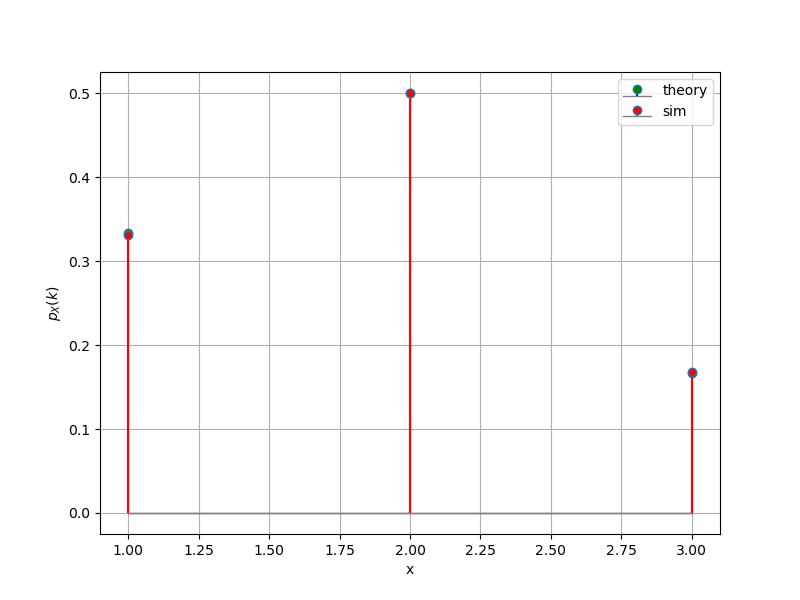
\includegraphics[width=\columnwidth]{figs/Q7_1.png}
		\caption{PMF plot}
		\label{stemplot}
	\end{figure}
	\begin{figure}[h!]
		\centering
		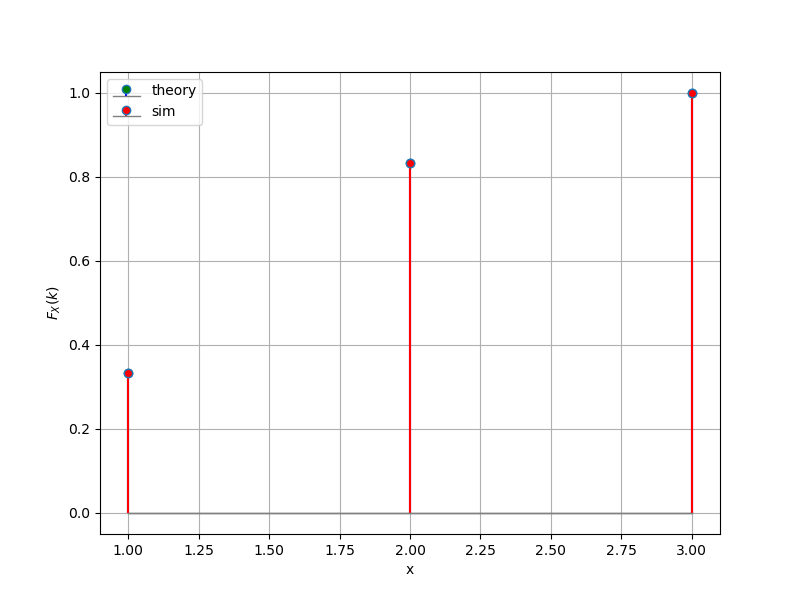
\includegraphics[width=\columnwidth]{figs/Q7_2.png}
		\caption{CDF plot}
		\label{stemplot}
	\end{figure}


\end{document}
